\documentclass{article}
\usepackage[english]{babel}
\usepackage[T1]{fontenc}
\usepackage[utf8]{inputenc}
\usepackage[a4paper, top=3cm,bottom=3cm,left = 2.9cm, right=2.9cm]{geometry}
\usepackage[infoshow,debugshow]{tabularx}
\usepackage{booktabs}
\usepackage{titlesec}
\usepackage{amsmath}
\usepackage{amssymb}
\usepackage{amsfonts}
\usepackage{amsthm}
\usepackage{xcolor}
\usepackage[bottom]{footmisc}
\usepackage[colorlinks=true, linkcolor=blue, citecolor=red, urlcolor=violet]{hyperref}
\usepackage{graphicx}
\usepackage{subcaption}
\usepackage{verbatim}
\usepackage{enumitem}
\usepackage{float}
\usepackage{chngcntr}
\usepackage{floatflt}
\usepackage{caption}
\newtheorem{theorem}{Theorem}[section]
\theoremstyle{remark}
\newtheorem{definition}{Definition}[section]
\theoremstyle{remark}
\newtheorem{proposition}{Proposition}[section]
\theoremstyle{definition}
\newtheorem{note}{Note}
\theoremstyle{definition}

% FIGURES can be defined here and then used or directly defined within the text
\def\trainUno{\centering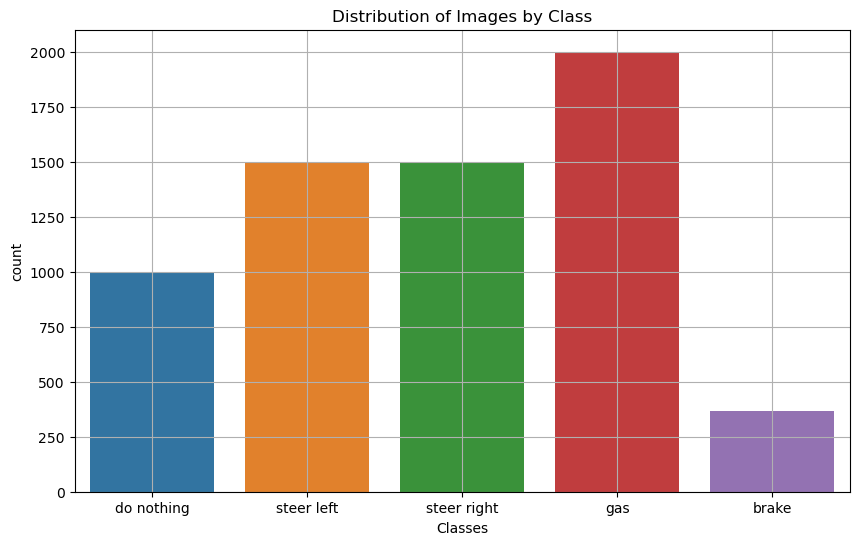
\includegraphics[width=0.7\textwidth]{img/trainUno.png}}
\def\trainDue{\centering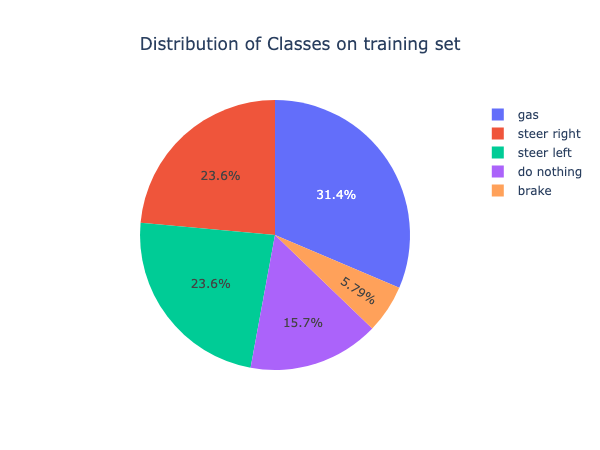
\includegraphics[width=1\textwidth]{img/trainDue.png}}
\def\testUno{\centering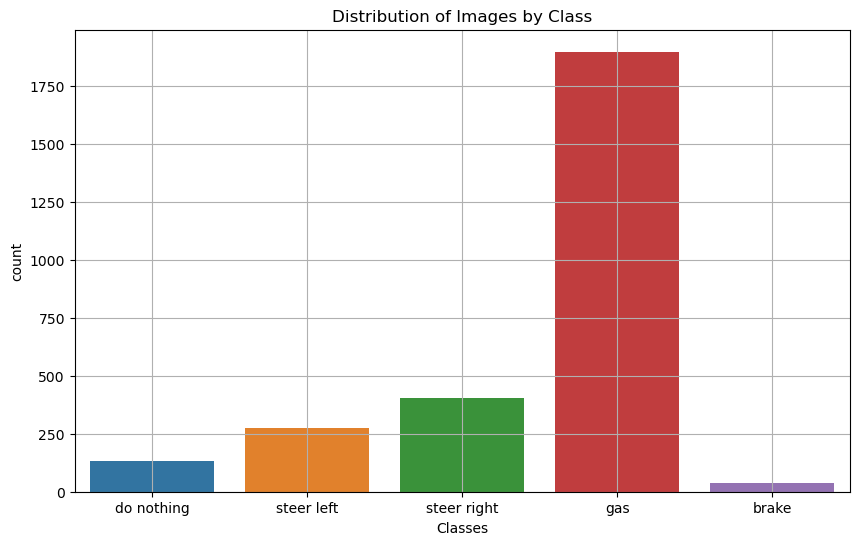
\includegraphics[width=0.7\textwidth]{img/testUno.png}}
\def\testDue{\centering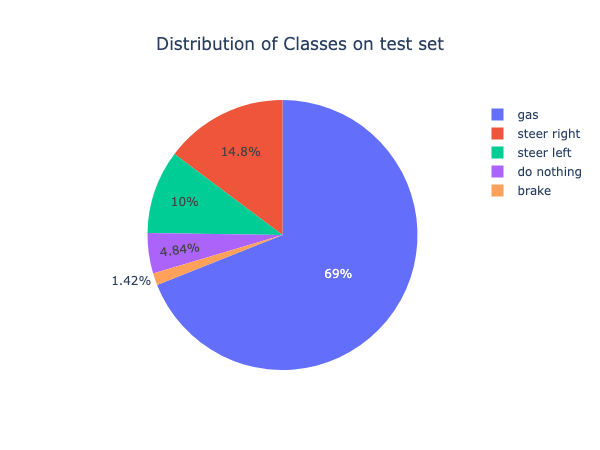
\includegraphics[width=1\textwidth]{img/testDue.png}}
\def\photo{\centering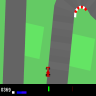
\includegraphics[width=0.4\textwidth]{img/photo.png}}
\def\photoPrep{\centering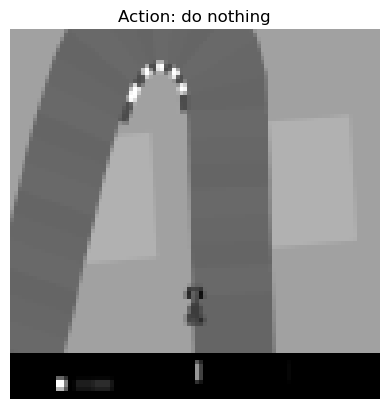
\includegraphics[width=0.4\textwidth]{img/photoPrep.png}}
\def\modA{\centering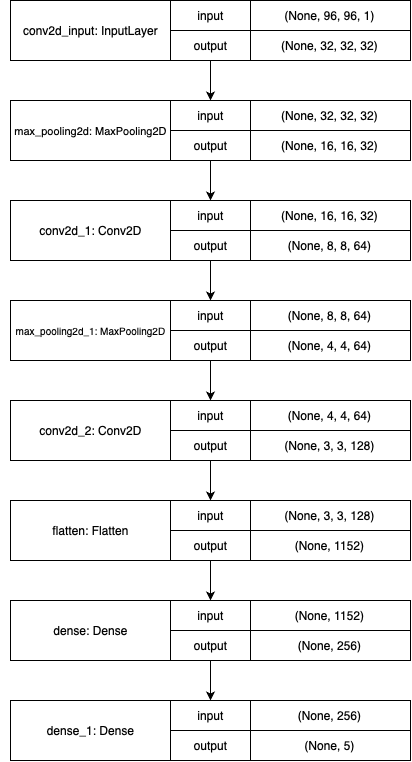
\includegraphics[width=0.4\textwidth]{img/modA.png}}
\def\modB{\centering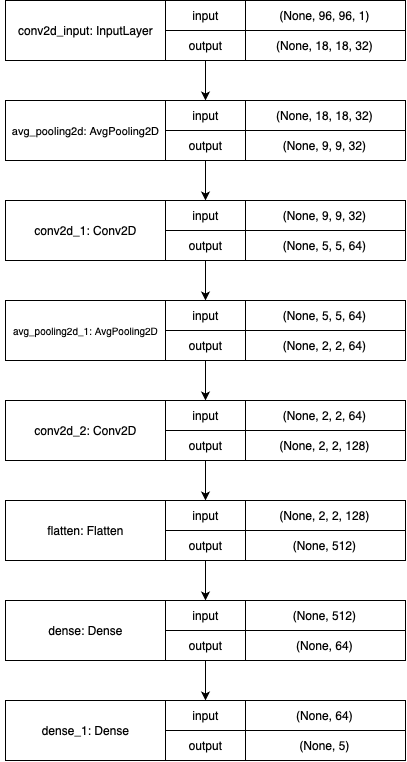
\includegraphics[width=0.4\textwidth]{img/modB.png}}
\def\weights{\centering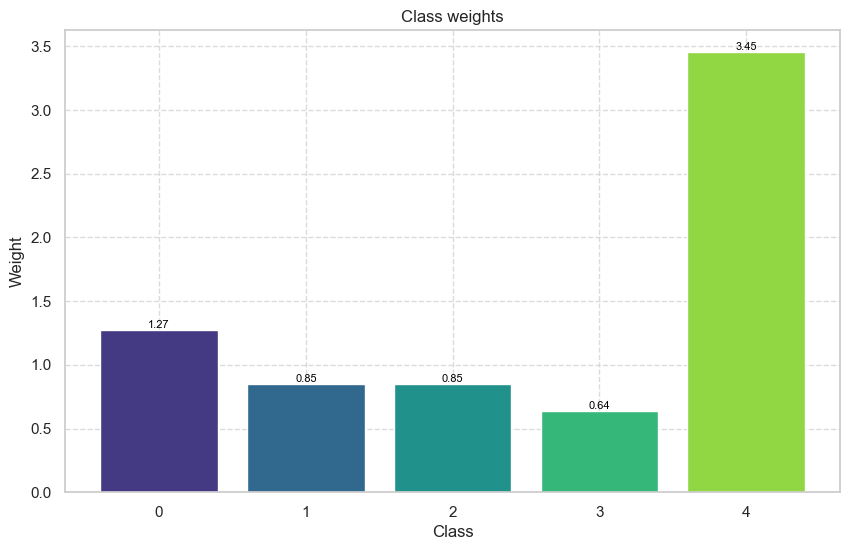
\includegraphics[width=0.6\textwidth]{img/weights.png}}
\def\testA{\centering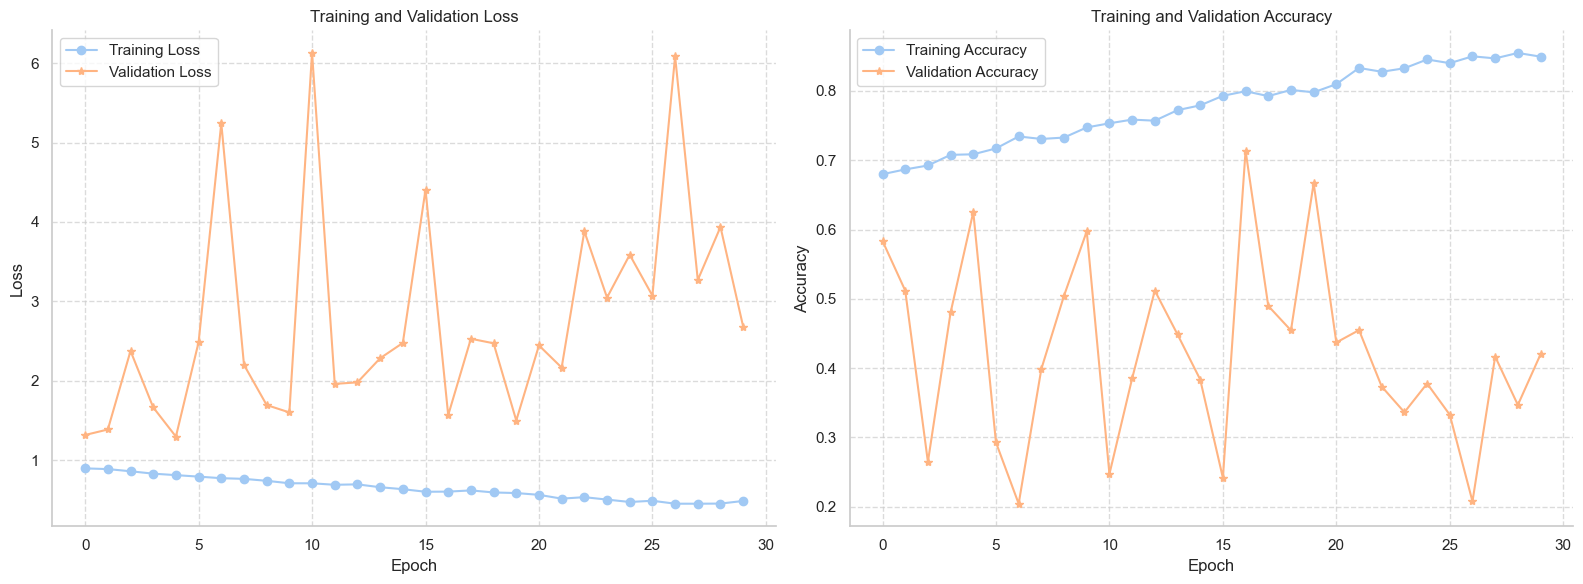
\includegraphics[width=0.8\textwidth]{img/testA.png}}
\def\CMA{\centering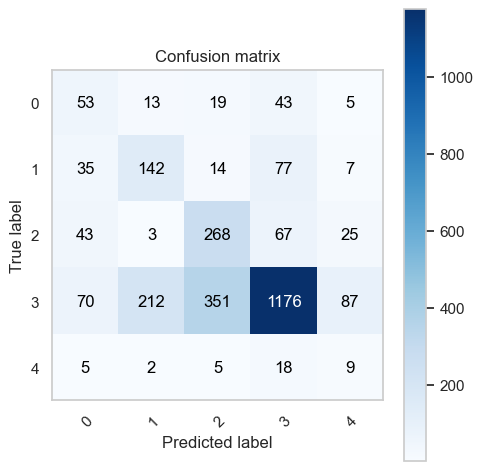
\includegraphics[width=0.5\textwidth]{img/CMA.png}}
\def\testB{\centering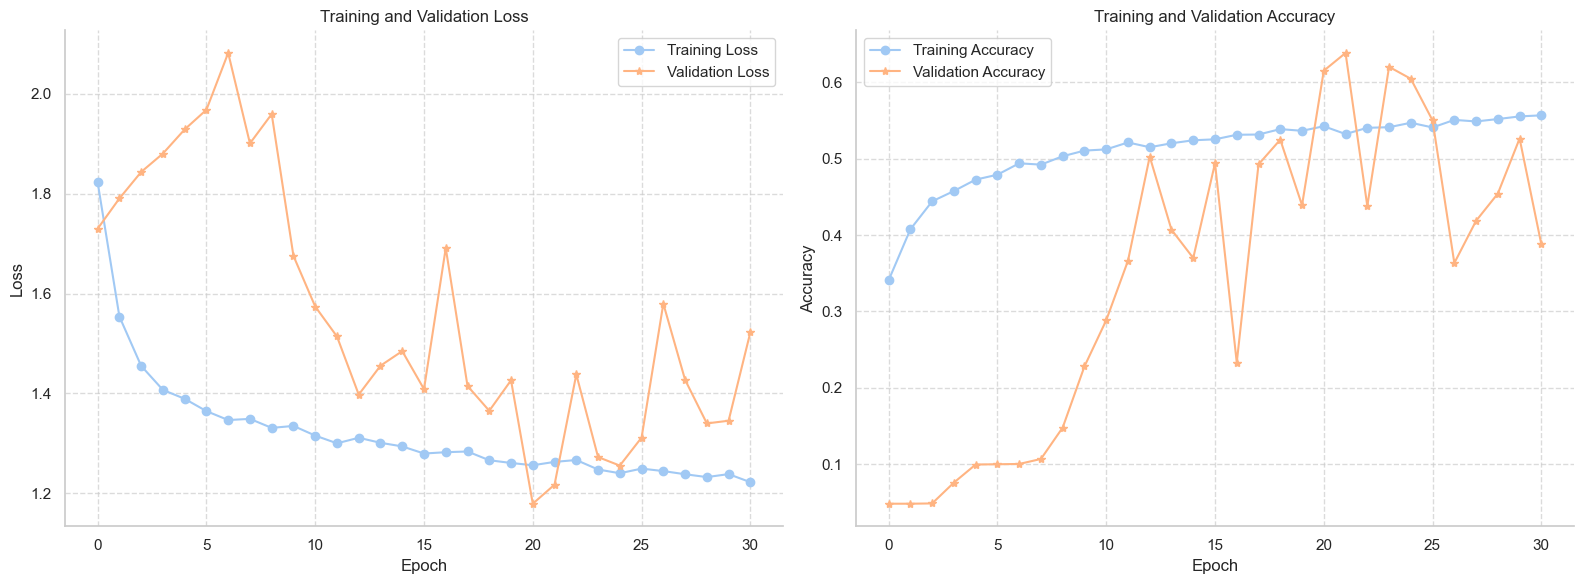
\includegraphics[width=0.8\textwidth]{img/testB.png}}
\def\CMB{\centering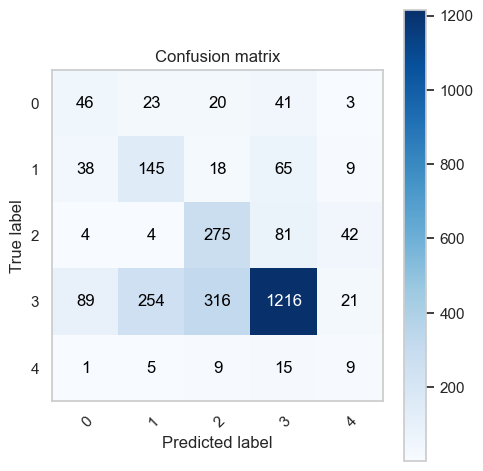
\includegraphics[width=0.5\textwidth]{img/CMB.png}}
\def\hUno{\centering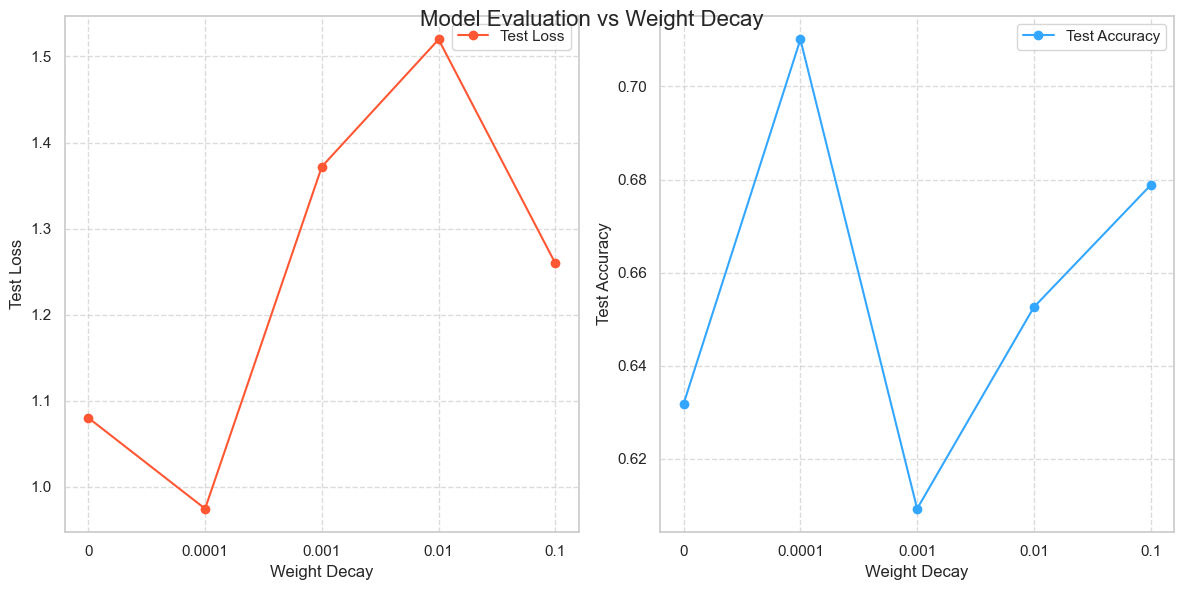
\includegraphics[width=0.8\textwidth]{img/h1}}
\def\hDue{\centering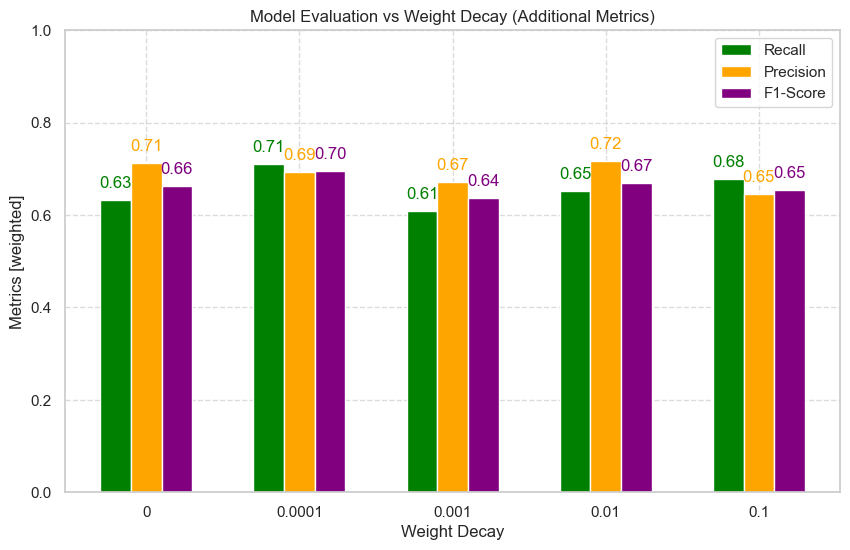
\includegraphics[width=0.5\textwidth]{img/h2}}

\title{Machine Learning \\ Homework 2}
\author{Simone Orelli\\ matricola 1749732}
\date{January 2024}

\begin{document}
\maketitle
\tableofcontents
	\section{Introduction}
In this homework, we are invited to solve an image classification problem to learn the behavior of a racing car in a Gym environment. For image classification problem we mean to analyze the image and identify the class (label) to which it belongs. This is one of the core problems in Computer Vision that, despite its simplicity, has a large variety of practical applications. Gym, launched by OpenAI, is an open-source bank of artificial intelligence projects. This database has been put together for developers to use various artificial intelligence techniques such as reinforcement learning and computer vision to solve these environments. The environment explored in this study was CarRacing-v0, a 2D autonomous vehicle environment. Using machine learning an agent was trained to learn this track.
	\section{Introduction}
In this homework, we are invited to solve an image classification problem to learn the behavior of a racing car in a Gym environment. For image classification problem we mean to analyze the image and identify the class (label) to which it belongs. This is one of the core problems in Computer Vision that, despite its simplicity, has a large variety of practical applications. Gym, launched by OpenAI, is an open-source bank of artificial intelligence projects. This database has been put together for developers to use various artificial intelligence techniques such as reinforcement learning and computer vision to solve these environments. The environment explored in this study was CarRacing-v0, a 2D autonomous vehicle environment. Using machine learning an agent was trained to learn this track.
	\subsection{The models}
The most commonly used image classification algorithm is the Convolutional Neural Network (CNN). A neural network is a function approximator represented by a parametric model. Given a target function $f$, the goal is to learn the parameters of the estimator \textbf{$\hat{f}(x,\Theta)$} in such a way that $\hat{f}$ results to be a good approximation of the target function $f$. Convolutional neural networks are a special class concerning feedforward (FNN) neural networks, where a FNN is an artificial neural network wherein connections between the nodes do not form a cycle: the information moves in only one direction, from the input through the hidden layers to the output. In its general form a neural net consists of a list of layers that transform the input volume into an output volume. The layers are divided into input layer, hidden layers and an output layer. Each layer accepts an input 3D volume and transforms it to an output 3D volume through a differentiable function. Typically, the input of a CNN is an image, the output is a vector defining the class to which the image belongs. The hidden layers are composed by the convolutional layers. Each convolutional layer is in turn composed of 3 stages:
\begin{itemize}
\item{\textbf{Convolution stage:} the convolution operation is defined as a translation of a matrix, called kernel, to the input matrix and represents a filter. The resulting matrix is generally smaller than the input matrix;}
\item{\textbf{Detector stage:} layer will apply an elementwise non-linear activation function, such as \textit{ReLU};}
\item{\textbf{Pooling stage:} layer will perform a downsampling operation along the spatial dimensions;}
\end{itemize}
As stated, in a convolutional neural network, the hidden layers include layers that perform convolutions. This is typically done by a layer that performs a dot product of the convolution kernel with the layer’s input matrix. As the convolution kernel slides along the input matrix for the layer, the convolution operation generates a feature map, which in turn contributes to the input of the next layer. The input is originally an image (tensor) with a shape: \textit{(input height) $\times$ (input width) $\times$ (input channels)}. After passing through a convolutional layer, the image becomes abstracted to a feature map with shape: \textit{(feature map height) $\times$ (feature map width) $\times$ (feature map channels)}. In a neural network, the number of parameters to tune grows rapidly with the increase of the number of layers (just think of a fully connected sequential net, if we have to connect $n$ units of a layer with $m$ units of the following one, we are adding $n \times m$ parameters to the model each time). Furthermore, in convolutional layers a parameter sharing scheme is used to control the number of free parameters. The result of convolution operations is an activation map, and the set of activation maps for each different filter are stacked together along the depth dimension to produce the output volume. To solve the image classification problem we will define two different models that share the same structure. The two models will be two CNN and they will differ from the structure.

\subsubsection{Model A}
In general, the structure of model A is composed of kernels that increase in layer after layer quantities. In particular they have medium sizes that decrease layer after layer. For the stride is worth a similar speech: it starts with a medium-sized stride that gradually decreases in size. As activation function is used Relu, as optimizer is used Adam and as pooling stage the Maximum Pooling is used. Finally, the network has two dense layers of connection. In the figure \ref{fig:modA} is shown its structure.
\begin{figure}[h!]
    \modA
    \caption{Architecture of the first model}
    \label{fig:modA}
\end{figure}
As shown in the figure \ref{fig:modA} we have $3$ convolutional layers (all of them have \textit{ReLU} as activation function):
\begin{itemize}
\item{\textbf{conv2d\_input:} this layer is composed by $32$ kernels of dimension $5 \times 5$ with stride $3 \times 3$ and same padding\footnote{\textbf{padding} represents the size of the outer edge applied to the input image; if 'same', padding is added so that the output has the same size as the original input.};}
\item{\textbf{conv2d\_1:} this layer is composed by $64$ kernels of dimension $3 \times 3$ with stride $2 \times 2$ and same padding;}
\item{\textbf{conv2d\_2:} this layer is composed by $128$ kernels of dimension $2 \times 2$ with stride $2 \times 2$ without padding;}
\end{itemize}
Then there are $2$ MaxPooling layers of $2 \times 2$ filters of stride $2$ and in the end there are $2$ FC (fully connected layers) followed
by a \textit{softmax} for output. Finally, we compile the model using Adam as optimizer\footnote{When building a model in a deep learning library like Keras, the optimizer is one of the key components that defines how the model will be trained. The optimizer is responsible for updating the model weights so as to reduce the cost function during training. In simpler terms, the optimizer determines how the model learns from the data during the training process. The choice of the optimizer can affect the convergence rate of the model, the ability of the model to exit from local minima, and its ability to generalize to new data.} with $0.001$ as learning rate.
In any case, to avoid overfitting, some regularization techniques have been implemented, such as:
\begin{itemize}
\item{\textbf{Batch Normalization:} Normalize the output of each layer so that it has a zero average and a unit standard deviation during training;}
\item{\textbf{Dropout}: During training, it randomly "deactivates" some neurons, forcing the network to develop more robust representations. In our case we have chosen $0.8$ as rate dropout;}
\item{\textbf{Weight decay:} Called also weight regularization, it is a technique that introduces a penalty to the weights of the model during training, helping to limit excessive growth. In practice, a penalty is added to the cost function during optimization. The term regularization of weights can be implemented in different forms, such as regularization $L1$ or $L2$. Regularization L1 adds the absolute sum of weights, while regularization L2 adds the sum of squares of weights. The addition of this penalty encourages the network to use smaller weights, thus reducing the complexity of the model and improving its generalization ability on unseen data. In our case we have implemented the regularization $L2$ (ridge) with rate equal to $0.001$;}
\end{itemize}
This model produces:
\begin{verbatim}
Total params: 349,573
Trainable params: 349,125
Non-trainable params: 448
\end{verbatim}

\subsubsection{Model B}
In general, the structure of model B is composed of kernels that increase in layer after layer quantities. In particular they start from large sizes that decrease layer after layer. For the stride is a similar matter: it starts with a large stride that gradually decreases in size. The Relu is used as an activation function,  SGD is used as an optimizer and Average Pooling is used as a pooling stage. Finally, the network has two dense layers of connection. In the figure \ref{fig:modB} is shown its structure.
\begin{figure}[h!]
    \modB
    \caption{Architecture of the second model}
    \label{fig:modB}
\end{figure}
As shown in the figure \ref{fig:modB} we have $3$ convolutional layers (all of them have \textit{ReLU} as activation function):
\begin{itemize}
\item{\textbf{conv2d\_input:} this layer is composed by $32$ kernels of dimension $11 \times 11$ with stride $5 \times 5$ and without padding;}
\item{\textbf{conv2d\_1:} this layer is composed by $64$ kernels of dimension $5 \times 5$ with stride $1 \times 1$ and without padding;}
\item{\textbf{conv2d\_2:} this layer is composed by $128$ kernels of dimension $3 \times 3$ with stride $1 \times 1$ and same padding;}
\end{itemize}
Then there are $2$ AvgPooling layers of $2 \times 2$ filters of stride $2$ and in the end there are $2$ FC (fully connected layers) followed
by a \textit{softmax} for output. Finally, we compile the model using SGD as optimizer with $0.001$ as learning rate.
In any case, to avoid overfitting, we have implemented the same regularization techniques implemented for model A:
\begin{itemize}
\item{\textbf{Batch Normalization:} Normalize the output of each layer so that it has a zero average and a unit standard deviation during training;}
\item{\textbf{Dropout}: rate dropout equal to $0.5$;}
\item{\textbf{Weight decay:} for model B was implemented the regularization $L2$ with rate equal to $0.001$;}
\end{itemize}
This model produces:
\begin{verbatim}
Total params: 163,077
Trainable params: 162,629
Non-trainable params: 448
\end{verbatim}
	\subsection{Results}
In this section we are going to explore the results reached by the two models. The results are evaluated in terms of driving performance of the car and in terms of accuracy, f1 score, precision and recall.
In order to evaluate the two models we have to fit they. The fitting is made by the function \verb+model.fit()+ where \verb+model+ is a \verb+sequential+ object of the \verb+keras.model+ library. The fit function is executed by setting $50$ epochs, $128$ batch size and by putting two techniques. One of them is useful for avoiding overfitting and the other is useful since we are working with an unbalanced training set. They are:
\begin{itemize}
\item{\textbf{Early stopping:} it's a technique used when training machine learning models to avoid overfitting. Its basic idea is to stop training when model performance on a validation set stops improving. In practice, the model is continuously evaluated on a validation data set during training, and if its performance does not improve for a number of consecutive epochs, training is interrupted. This technique is useful to prevent the trained model from learning the training data too well, adapting to noises or peculiarities specific to that data set but losing the ability to generalize to new unseen data. Early stopping helps to find the optimal point where the model has the best performance on validation data. In our case we have implemented the early stopping with $10$ as patience and it is started after the first $15$ epochs;}
\item{\textbf{Class weight:} it's a technique used when working with unbalanced datasets, in which some classes have significantly more or fewer examples than other classes. In this context, assigning different weights to classes during training can help the model to give greater importance to the less represented classes. When class weight is used, a different weight can be assigned to each class when filling in the model. For example, if a class has fewer examples, its weight can be increased, while for a class with more examples the weight can be reduced. This allows the model to "pay more attention" to the less represented classes during training. The use of class weight is useful when you want to ensure that the model is not dominated by the majority classes and that it is able to generalize well even on less represented classes. In our case we have chosen the weights shown in the figure \ref{fig: weights};
\begin{figure}[h!]
    \weights
    \caption{Class weights}
    \label{fig: weights}
\end{figure}}
\end{itemize}

\subsubsection{Model A}
For fitting the first model we need of 48.3 seconds. The results are evaluated using the cross entropy loss function and accuracy. The results are shown in figure \ref{fig:testA}.
\begin{figure}[h!]
    \testA
    \caption{Test and Loss accuracy for model A}
    \label{fig:testA}
\end{figure}
In particular, for the first model we have:
\begin{verbatim}
Test loss: 1.4987
Test accuracy: 0.6668
\end{verbatim}
It can be noted that this model is affected by overfitting despite the various regularization techniques applied. This can be seen by observing the trend of the accuracy curves on the training set and test set. In particular, you can see that the accuracy curve on the training set increases without the test curve actually converging. This means that the model has learned and adapted too well to the training data, but struggles to generalize well to new unseen data. To heal our model from overfitting one might consider to apply data augmentation on training set, in order to expand the dataset and improve the model generalization. Another idea might be to reduce the learning rate to make optimization more stable and allow the model to converge better however without exaggerating otherwise the model might suffer from underfitting\footnote{Underfitting is a condition in which a machine learning model fails to adequately capture the complexity of training data, leading to unsatisfactory performance on both training and test data. In other words, the model is too simple to correctly represent the relationship between input and output variables in your problem.}. Otherwise you might think of adding more dropout layers and/or batch normalization layers in the model. The classification report is:
\begin{verbatim}
              precision    recall  f1-score   support

         0.0       0.20      0.23      0.21       133
         1.0       0.31      0.48      0.38       275
         2.0       0.58      0.37      0.45       406
         3.0       0.79      0.80      0.80      1896
         4.0       0.31      0.10      0.15        39

    accuracy                           0.67      2749
   macro avg       0.44      0.40      0.40      2749
weighted avg       0.68      0.67      0.67      2749
\end{verbatim}
Finally, in figure \ref{fig:CMA} is shown the confusion matrix of this model.
\begin{figure}[h!]
    \CMA
    \caption{Confusion matrix for model A}
    \label{fig:CMA}
\end{figure}

\subsubsection{Model B}
For fitting the first model we need of $58.1$ seconds and the results are shown in figure \ref{fig:testB}.
\begin{figure}[h!]
    \testB
    \caption{Test and Loss accuracy for model B}
    \label{fig:testB}
\end{figure}
In particular, for the first model we have:
\begin{verbatim}
Test loss: 1.1791
Test accuracy: 0.6151
\end{verbatim}
We can see that this model is affected by overfitting less than the first.
The classification report is:
\begin{verbatim}
              precision    recall  f1-score   support

         0.0       0.26      0.35      0.30       133
         1.0       0.34      0.53      0.41       275
         2.0       0.43      0.68      0.53       406
         3.0       0.86      0.64      0.73      1896
         4.0       0.11      0.23      0.15        39

    accuracy                           0.62      2749
   macro avg       0.40      0.48      0.42      2749
weighted avg       0.70      0.62      0.64      2749
\end{verbatim}
Finally, in figure \ref{fig:CMB} is shown the confusion matrix of this model.
\begin{figure}[h!]
    \CMB
    \caption{Confusion matrix for model B}
    \label{fig:CMB}
\end{figure}
	\section{Introduction}
In this homework, we are invited to solve an image classification problem to learn the behavior of a racing car in a Gym environment. For image classification problem we mean to analyze the image and identify the class (label) to which it belongs. This is one of the core problems in Computer Vision that, despite its simplicity, has a large variety of practical applications. Gym, launched by OpenAI, is an open-source bank of artificial intelligence projects. This database has been put together for developers to use various artificial intelligence techniques such as reinforcement learning and computer vision to solve these environments. The environment explored in this study was CarRacing-v0, a 2D autonomous vehicle environment. Using machine learning an agent was trained to learn this track.
\end{document}